\documentclass[prodmode,acmtecs]{acmsmall}

\usepackage[ruled]{algorithm2e}
\renewcommand{\algorithmcfname}{ALGORITHM}
\SetAlFnt{\small}
\SetAlCapFnt{\small}
\SetAlCapNameFnt{\small}
\SetAlCapHSkip{0pt}
\IncMargin{-\parindent}

% Metadata Information
\acmVolume{9}
\acmNumber{4}
\acmArticle{39}
\acmYear{2010}
\acmMonth{3}

% Document starts
\begin{document}

% Page heads
\markboth{A. Biancini et al.}{Shibboleth suthentication for non-web application}

% Title portion
\title{Shibboleth authentication for non-web application}
\author{ANDREA BIANCINI
\affil{INFN - Sezione Milano Bicocca\\andrea.biancini@mib.infn.it}
FABIO FARINA
\affil{Consortium GARR\\fabio.farina@garr.it}
SIMON VOCELLA
\affil{Consortium GARR\\simon.vocella@garr.it}}

%Abstract
\begin{abstract}
Abstract Lorem ipsum dolor sit amet, consectetur adipisicing elit, sed do eiusmod tempor incididunt ut labore et dolore magna aliqua.
Ut enim ad minim veniam, quis nostrud exercitation ullamco laboris nisi ut aliquip ex ea commodo consequat.
Duis aute irure dolor in reprehenderit in voluptate velit esse cillum dolore eu fugiat nulla pariatur.
Excepteur sint occaecat cupidatat non proident, sunt in culpa qui officia deserunt mollit anim id est laborum.
Lorem ipsum dolor sit amet, consectetur adipisicing elit, sed do eiusmod tempor incididunt ut labore et dolore magna aliqua.
Ut enim ad minim veniam, quis nostrud exercitation ullamco laboris nisi ut aliquip ex ea commodo consequat.
Duis aute irure dolor in reprehenderit in voluptate velit esse cillum dolore eu fugiat nulla pariatur.
Excepteur sint occaecat cupidatat non proident, sunt in culpa qui officia deserunt mollit anim id est laborum.
Lorem ipsum dolor sit amet, consectetur adipisicing elit, sed do eiusmod tempor incididunt ut labore et dolore magna aliqua.
Ut enim ad minim veniam, quis nostrud exercitation ullamco laboris nisi ut aliquip ex ea commodo consequat.
Duis aute irure dolor in reprehenderit in voluptate velit esse cillum dolore eu fugiat nulla pariatur.
Excepteur sint occaecat cupidatat non proident, sunt in culpa qui officia deserunt mollit anim id est laborum.
Lorem ipsum dolor sit amet, consectetur adipisicing elit, sed do eiusmod tempor incididunt ut labore et dolore magna aliqua.
Ut enim ad minim veniam, quis nostrud exercitation ullamco laboris nisi ut aliquip ex ea commodo consequat.
Duis aute irure dolor in reprehenderit in voluptate velit esse cillum dolore eu fugiat nulla pariatur.
Excepteur sint occaecat cupidatat non proident, sunt in culpa qui officia deserunt mollit anim id est laborum.

\end{abstract}

\category{C.2.2}{Computer-Communication Networks}{Network Protocols}

\terms{Shibboleth, PAM, JAAS}

\keywords{Shibboleth, SAML, Basic authentication, PAM, JAAS, Python}

\acmformat{Biancini A., Farina F., Vocella S. 2012. Shibboleth authentication for non-web application.}

%\begin{bottomstuff}
%This work is supported by the National Science Foundation, under
%grant CNS-0435060, grant CCR-0325197 and grant EN-CS-0329609.
%
%Author's addresses: G. Zhou, Computer Science Department,
%College of William and Mary; Y. Wu  {and} J. A. Stankovic,
%Computer Science Department, University of Virginia; T. Yan,
%Eaton Innovation Center; T. He, Computer Science Department,
%University of Minnesota; C. Huang, Google; T. F. Abdelzaher,
%Computer Science Department, University of Illinois at Urbana-Champaign.
%\end{bottomstuff}

\maketitle

%Body text of the article
\label{sec:introduction}
\section{Introduction}
User authentication and user authorization are main tasks needed to guarantee security in IT environments.
One important requirement of such security solutions, is that they must be as transparent as possibile.
Current user applications, usually sit on different systems and environment.
This requires a solution able to permit that each system is not required to create and manage its own credential system.
For this reason single sign-on (SSO, as described in \cite{Shaer-1995}) systems have been designed and implemented.
These systems have also a strong impact on users who don't need to perform multiple logins on different systems, but could be automatically
identified by all the application they are using.\\
\\
One of the most widespread SSO software package is Shibboleth \cite{Morgan-2004}, which implements authentication and authorization over
network resources with a federated approach.
Shibboleth, designed and implemented by Internet2, provides an effective solution for secure multi-organizational access to web resources.
It implements widely used federated identity standards, principally OASIS' Security Assertion Markup Language (SAML \cite{Cantor-2005}), to
provide a federated single sign-on and attribute exchange framework.
Shibboleth also provides extended privacy functionality allowing the browser user and their home site to control the attributes released to
each application.\\
\\
Using Shibboleth-enabled access simplifies the management of identity and permissions for organizations supporting either users or
applications.
Shibboleth is developed in an open and participatory environment and is freely available.
This open and collaborative nature has allowed Shibboleth to become the heart of many solutions for single sign-on and Authentication \&
Authorization Infrastructures (AAI) in several identity federations.\\
\\
The architecture of Shibboleth, described in \cite{Erdos-2005}, identifies two main components: Identity Providers (IdPs) which authenticate
the users and supply user authorization attributes; Service Providers (SPs) which consume user attributes and provide access to the secure
contents.\\
The communication excanges between the user, the IdP and the SP are all base don SAML assertions and transit over HTTP channels.
This implementation architecture permits Shibboleth to works seamlessly inside user web-browsers.
However, this approach is strongly web-centric, and for this reason does not adapt well to provide SSO authentication to non web-based
application.\\
\\
In this article a solution is presented to permit Shibboleth authentication for non web-based applications.
The traditional login scheme used by Shibboleth to authenticate users is implemented inside a web-borser.
The user, when trying to log to a web resources, is redirected to the IdP to perform authentication and obtain authorization assertions via
his session metadata.
The use case implemented within this article solves the problem of authenticatin a user and retrieving his metadata information from Shibboleth
without using a web-broser.
This solution could be integrated in traditional client-based application (for instance application written in Java or Python) to obtain
a secure way to manager user logins.\\
\\
This article will describe the architecture and the technical implementation of this authentication solution.
As an example of possible uses of this work, different software implementations will be described showing how to integrate the shibboleth AAI
mechanisms inside several client applications (Linux platform, Java JAAS, Python).\\
\\
The rest of this paper is organized as follows: the first section contains a quick overview of related works; the second section will present
the architecture of the solution presented with this article; the third section will present some details about the technical implementation
in the different software platform; the last section presents conclusions and future works.

\label{sec:relatedworks}
\section{Related works}
To solve this problem of AAI integration between Shibboleth and non-web application the more general and wide approach is the Moonshot
project (\cite{Howlett-2010}).
This project aims explicitly to develop a single unifying technology for extending the benefits of federated identity to a broad range of
non-Web services.
The Moonshot project proposes a solution to the AAI problem very complete and articulated.\\
It leverages different technologies such as Kerberos (a computer network authentication protocol which allows nodes communicating over a
non-secure network to prove their identity to one another in a secure manner), the GSS library (Generic Security Services libraries for
programs to access security services) and a Radius server (Remote Authentication Dial In User Service, a networking protocol that provides
centralized Authentication, Authorization, and Accounting management).\\
This solution is for sure very complete and trusthworty.
It implies however a quite complex architecture and requires a lot of changes on client side, SPs and IdPs.
This suggests a difficult introduction of this approach into real existing federations.\\
\\
The need to leverage Shibboleth identity federations in non-web application has been particularly felt in Grid Computing
(\cite{Kesselman-1998}) services.
In the field of research, in fact, in the last years strong investments have been done to build a global e-Infrastructure leveraging Grid
Computing technologies.
This infrastructure supports the execution of scientific computation and the storage of relevant research data.\\
The grid, since its inception, has introduced specific solutions (inspired to the original article \cite{Foster-1998}) to security problems.
The new Shibboleth SSO for web-application somehow lies next to the Grid AAI, thus the idea to integrate the two security systems is natural
and potentially very beneficial.\\
Due to the complexity of the Moonlite project, which would add to the intrinsic complexity of grid security schemas, different solutions have
been adopted in this field.
\\
In grid environments, this problem has been approached with the goal to try and integrate the existing grid security infrastructures with
Shibboleth mechanisms.
These solutions, described in both articles \cite{Wang-2009} and \cite{Jensen-2007}, permit the users to transparently move between Shibboleth
application and Grid environments using one single set of credentials.
They work with specific software middlewares able to log in the user and then manage both the Shibboleth authentication assertions and the
grid certificates used to access the different environments where applications sit.\\
Solutions like those, are very interesting in that they really ease the user experience and provide effective results.
However it must be noted that are well fit for the problem of integrating Shibboleth with grid security and can hardly be extended to other
fields of application.
They are not able to provide a solution for the AAI needs of non-web application not running on a grid environment.\\
\\
The approaches described show opposite characteristics.
On one side a very complex and articulated mechanism has been proposed, on the other side very specific and poorly adaptable solutions
have been proposed to solve pragmatic problems.\\
In this paper a different approach will be presented.
The proposed approach would try and address general problems of authentication, but will try to do it with few interventions on the
requirements of SPs and IdPs.

\label{sec:architecture}
\section{Architecture}
The solution proposed leverages the standard authentication and authorization mechanisms implemented in Shibboleth.
It executes a login to the IdP using HTTP Basic mechanism (\cite{Franks-1999}) over https.
The authentication process of Shibboleth works as described in figure \ref{fig:shiblogin}.

\begin{figure}[h]
\centering
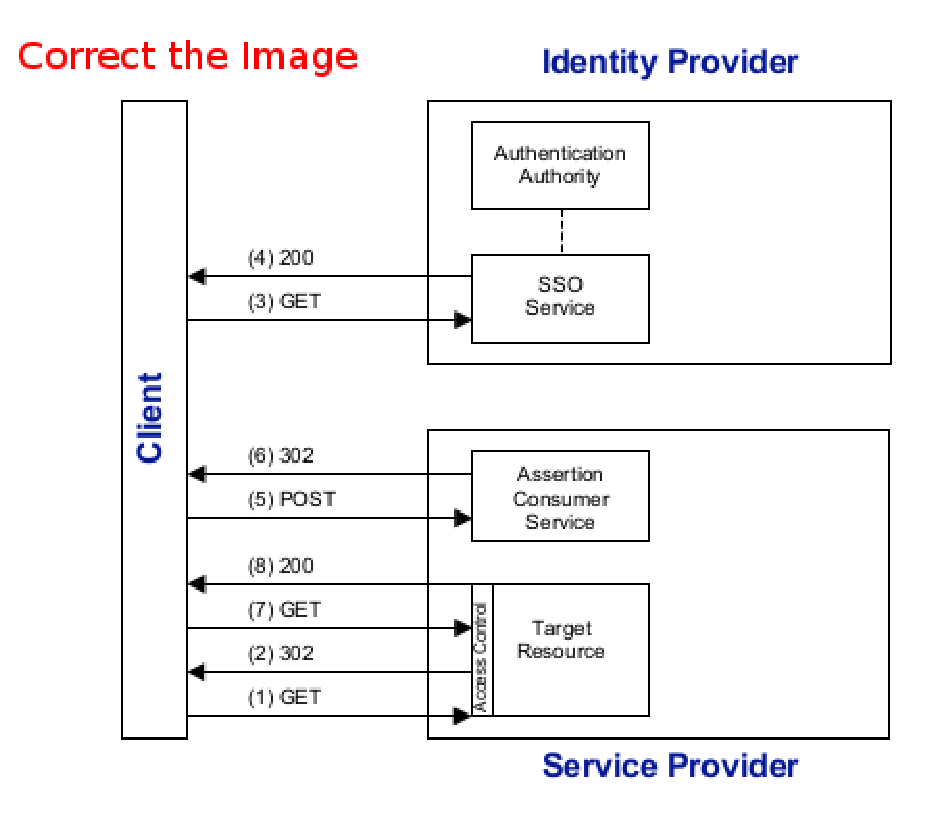
\includegraphics[width=8cm]{Fig1shiblogin.eps}
\caption{Shibboleth login procedure}
\label{fig:shiblogin}
\end{figure}

The solution described in this article follows the same schema, but with the following clarifications:
\begin{enumerate}
\item The original request is directed to a web-page on the SP side that is behind Shibboleth authentication.
This page will produce a list of rows key=value containing the metadata information to be passed to user session after login.
\item The webserver on the SP answers with a redirect operation to a page on the IdP.
\item The client follows the redirect and opens the IdP login page.
\item This request obtains an answer ``authorization required" asking the client to autenticate via HTTP Basic.
\item The client authenticates performing the same request with the proper HTTP header containing username and password for the user.
The answer to this request contains a Set-Cookie instruction with which the IdP creates a cookie on the client containing a couple of
keys permitting the client to reconnect with the Shibboleth session created.
\item The IdP communicates with the SP to create a valid session for the user with all the metadata of the user session.
\item The client opens the original URL providing the cookie set by the IdP after the authentication.
This requeste gets the page with the key=value rows used to initialize the user session on the client side.
\end{enumerate}

This mechanism simulates what usually happens in the browser of a user authentication to a Shibboleth web-application.
All this interactions are, however, automatic and do not require a user to manage or control the underlying HTTP dialogue to permit the
authentication.\\
\\
In order for this mechanism to work, a web page has been created on a server and placed behind Shibboleth authentication.
The user, after having provided valid login information, is shows this page that consists of a list rows with the format key=value.
This list represents the user session and shows all the relevant metadata provided by Shibboleth with the user authentication.
An example of the content of this page is as follows:
\begin{algorithm}[t]
\SetAlgoNoLine
\texttt{authenticated=true}\\
\texttt{Shib-Application-ID=default}\\
\texttt{Shib-Session-ID=\_d28ec2af03fd7437ca500c351ab0aec0}\\
\texttt{Shib-Identity-Provider=http://idp.server.hosntame/idp/shibboleth}\\
\texttt{Shib-Authentication-Instant=2012-06-15T12:55:45.587Z}\\
\texttt{Shib-Session-Index=0141d3c23dc19ee047f68e35037828a9db68d7961082566c9b399e512e03705f}\\
\texttt{eduPersonEntitlement=urn:mace:mib.infn.it:permission:service1:access:user}\\
\texttt{eduPersonPrincipalName=user@domain.it}\\
\texttt{eduPersonScopedAffiliation=member@domain.it;student@domain.it}\\
\texttt{eduPersonTargetedID=http://idp.server.hosntame/idp/shibboleth!https://sp.server...}\\
\texttt{email=name.surname@domain.it}\\
\texttt{givenName=Name}\\
\texttt{sn=Surname}\\
\texttt{uid=name}\\
\texttt{Shib-Session-Unique=64656661756c7468747470733a2f2f636c6f75642d6d692d30332e6d696...}
\caption{Example of PAM webpage on the S}
\label{alg:examplepam}
\end{algorithm}

\label{sec:implementations}
\section{Implementations}
This article will present different implementations of this AAI solution.
In order to test it in different scenarios and a wide spectrum of application, a set of different implementations have been realized
covering the more widespread application platforms.\\
\\
In particular three main implementations have been realized: an integration of these authorization and authentication mechanisms inside
Linux PAM and NSS modules; a integration with Java JAAS architecture; a module for python applications.
In the following part of this section, these implementations will be described.

\label{sec:pamnss}
\subsection{PAM and NSS modules}
The standard mechanisms used by modern Linux systems to authenticate and list users are PAM and NSS.
These two libraries have different purposes and implement different functionalities.

\label{sec:pam}
\subsubsection{Pluggable Authentication Modules (PAM)}
Pluggable Authentication Modules (PAM) are at the core of user authentication in any modern linux distribution.
PAM enables the user programs to transparently authenticate users, regardless of how security information is stored.
As described in the Linux-PAM System Administrator's Guide (\cite{Morgan-1996}): ``It is the purpose of the Linux-PAM project to separate
the development of privilege granting software from the development of secure and appropriate authentication schemes.
This is accomplished by providing a library of functions that an application may use to request that a user be authenticated".\\
\\
For this reason, in order to guarantee a SSO mechanism on linux machines it seemed straightforward to implement a module for
PAM able to authenticate and retrieve user sessions from Shibboleth via the HTTP Basic authentication mechanism.
In order to authenticate using HTTP Basic, the general schema presented in secion \ref{sec:architecture} is implemented using the
libcurl library (\cite{Stenberg-1996}).\\
Libcurl is used to manage all the HTTP dialogues and is able to manage cookies and perform the HTTP basic authentication, when
required by the IdP.
\\
A PAM module is a shared library with a public interface, specified by PAM headers, that links with the user programs to perform
actions of authentication, accounting and to retrieve user session values.
The methods that needs to be implemented are the following:
\begin{itemize}
\item \texttt{pam\_sm\_authenticate}: this function performs user authentication.
This function has to request to the user his user ID and password.
To perform these operation the PAM library uses an application-defined callback to allow a direct communication between a loaded module
and the user via the application.\\
This function, retrieved, the needed information, starts the login procedure with the SP and IdP and provides an answer wether the user
has been able to provide a valid authentication or not.
\item \texttt{pam\_sm\_setcred}: this function retrieves information to create a session for the user.
Generally, an authentication module may have access to more information about a user than their authentication token.
This function is used to make such information available to the application.
The session values are obtained from the web page used to perform HTTP Basic authentication.
As described in section \ref{sec:architecture}, this page contains in fact a list of key=value rows retrieving information from Shibboleth
metadata and describing the logged user session.
\item \texttt{pam\_sm\_acct\_mgmt}: this function performs the task of establishing whether the user is permitted to gain access at this time.
This function gets called when the user has already been validated by an authentication module.
This function checks for the returned page body of the HTTP target resources behind Shibboleth authentication to verify that the
\texttt{authenticate} variable is specified with value \texttt{true}.
\item \texttt{pam\_sm\_open\_session}: this function is called to commence a session.
\item \texttt{pam\_sm\_close\_session}: this function is called to terminate a session.
\item \texttt{pam\_sm\_chauthtok}: this function is used to (re-)set the authentication token of the user.
This function is not implemented in the module realized for Shibboleth.
In fact the PAM module realized is not able to modify user information on the IdP side but it is used only to chech user session and
perform AAI.
\end{itemize}

This PAM module developed, can then be used to authenticate users in a common PAM chain.
For example, modifying the file \texttt{/etc/pam.d/login} and modyfing with the config file in algorithm \ref{alg:pamconf}, it is
possible to permit login to the linux machine using the Shibboleth credentials.\\
The \texttt{pam\_http.so} module can be instatiated with some parameters.
In particular, it is possible to specify the following parameters:
\begin{itemize}
\item url: specifies the URL of the page behind Shibboleth authentication on the SP that produces as output the data to be put in user
session after login;
\item sess\_username: specifies the field in the user session containing the username to be passed to the system for the logged in user;
this name, in the standard linux process, can differ from the one used for login;
\item sslcheck (optional): specifies whether the libcurl library has to verify the SSL certificate of the server when connecting via HTTPS;
\item cafile (optional): specifies the name of a file, containing a CA public key, used by libcurl to verify the SSL certificate of the server
when connecting via HTTPS.
\end{itemize}

\begin{algorithm}[t]
\SetAlgoNoLine
\texttt{auth     required       pam\_http.so url=https://servername.com/pam sess\_username=username}\\
\texttt{account  required       pam\_http.so}\\
\texttt{password required       pam\_permit.so}\\
\texttt{session  required       pam\_http.so}
\caption{PAM configuration to use the \texttt{pam\_http} module.}
\label{alg:pamconf}
\end{algorithm}

\label{sec:nss}
\subsubsection{Name Service Switch (NSS)}
To permit a linux system to user external directories for users and user groups, it is necessary to implement another module for a different
library: the Name Service Switch (NSS, \cite{GNU-1987}).
This library permits to define services for accessing different databases containing various information.
In respect of the activites described in this article, the relevant databases are: \texttt{passwd}, the user dadatabase; and \texttt{group}
a database with all user groups.\\
\\
The service implemented to integrate NSS with Shibboleth is a new servlet that has been deployed on the IdP.
This servlet connects to the underlying authorization database (usually an LDAP database) and retrieves information about all users and groups
that are recognized by that IdP.\\
\\
The NSS module implemented, than, had to implement the following functions:
\begin{itemize}
\item \texttt{\_nss\_shib\_getpwnam\_r}: this function is called to retrieve user information starting from his user-name;
\item \texttt{\_nss\_shib\_getpwuid\_r}: this function is called to retrieve user information starting from his uid;
\item \texttt{\_nss\_shib\_getpwent\_r}: this function is called to retrieve all the available users;
\item \texttt{\_nss\_shib\_getgrnam\_r}: this function is called to retrieve a user group information starting from its name;
\item \texttt{\_nss\_shib\_getgrgid\_r}: this function is called to retrieve a user group information starting from its id (gid);
\item \texttt{\_nss\_shib\_getgrent\_r}: this function is called to retrieve all the available user groups.
\end{itemize}

This NSS module can be activated by modyfing the \texttt{/etc/nsswitch.conf} file as shown in algorithm \ref{alg:nssconf}.
The NSS module reads some configuration form the configuration file \texttt{/etc/libnss.conf}.
In particular, it is possible to specify the following parameters:
\begin{itemize}
\item url: specifies the URL of the servlet created on the IdP and able to list users and groups of users of a specific identity provider;
\item sslcheck (optional): as for the PAM module, specifies whether the libcurl library has to verify the SSL certificate of the server when
connecting via HTTPS;
\item cafile (optional): as for the PAM module, specifies the name of a file, containing a CA public key, used by libcurl to verify the SSL
certificate of the server when connecting via HTTPS;
\item username (optional): if the servlet is behind an authentication method, specifies the username to be used for login;
\item password (optional): if the servlet is behind an authentication method, specifies the password to be used for login;
\item cookie\_num: specifies the number of cookies to be passed to the servlet; if no cookie has to be passed, 0 must be specified here;
\item coolie\_\#\_name: specifies for each cookie the name of the cookie to be passed; values with \$\{name\} are considered variables to
be searched in the environment;
\item coolie\_\#\_value: specifies for each cookie the value of the cookie to be passed; values with \$\{name\} are considered variables to
be searched in the environment.
\end{itemize}

\begin{algorithm}[t]
\SetAlgoNoLine
\texttt{passwd:     files shib}\\
\texttt{shadow:     files}\\
\texttt{group:      files shib}\\
\texttt{}\\
\texttt{hosts:      files dns}
\caption{NSS configuration to use the \texttt{shib} module.}
\label{alg:nssconf}
\end{algorithm}

With this two modules the linux machine recognizes Shibboleth users in the same way as local users.
So a Shibboleth user can login to the linux machine with his credentials, can have access rights on files, use ACLs, and so on...\\
\\
After the login the user finds in its login environment all the Shibboleth session values.
All metadata downloaded from Shibbolet is in fact placed in the user session and can be used to perform SSO with other non web-based
application.

\label{sec:jaas}
\subsection{JAAS module}
Java, with its Enterprise Edition, has become a very well known and ubiquitous platform for developing software applications.
Starting from Java 1.4 a common service has been introduced for AAI: the Java Authentication and Authorization Service (JAAS,
\cite{Java-2002}).
JAAS can be used for two purposes:
\begin{itemize}
\item for authentication of users, to reliably and securely determine who is currently executing Java code, regardless of
whether the code is running as an application, an applet, a bean, or a servlet; and
\item for authorization of users to ensure they have the access control rights (permissions) required to do the actions
performed.
\end{itemize}

JAAS implements a Java version of the standard Pluggable Authentication Module (PAM) framework.
For this reason, and for its widespread utilization in real applications, JAAS seemed a proper candidate to integrate a module
to authenticate users on Shibboleth.
Via this module it is now possible to integrate Shibboleth authentication, and metadata management, inside Java application
not based on web-technologies.\\
\\
The general architecture of this JAAS module is the same of the PAM module described in this article in section \ref{sec:pam}.
A JAAS module is implemented by a class extending the \texttt{javax.security.auth.spi.LoginModule} class and implementing
the following methods:

\begin{itemize}
\item \texttt{initialize}: this method is used to initialize the login module specifying: the subject to be authenticated,
a callback handler to deal the communications with the end user (in a very similar way to PAM conversation mechanisms);
\item \texttt{login}: this method authenticates the user by checking his user name and password;
\item \texttt{logout}: this method logs out the user;
\item \texttt{abort}: this method is called if the login process terminates for some reason internal to JAAS configuration
and cleans up any state that was originally saved;
\item \texttt{commit}: this method is called if the login process concludes positively; it associates a set of principals
to the login context; these principals can contain relevant information about the user session.\\
Within the JAAS module for Shibboleth a specific principal has been developed (the \texttt{ShibbolethPrincipal}).
This principal contains a \texttt{Map<String, String>} object that represents the user session containing all Shibboleth
metadata information.
\end{itemize}

This JAAS module can be configured with a configuration file as the one presented in algorithm \ref{alg:jaasconf}.
The login module accepts the same parameter of the PAM module described in section \ref{sec:pam} but,
instead of having \texttt{cafile}, has a mechanism to authenticate server SSL certificates that leverages the standard
trustsotres of Java defined by specifying the truststore file name and the password to access it.

\begin{algorithm}[t]
\SetAlgoNoLine
\texttt{Shibboleth \{}\\
\texttt{  it.infn.mib.shibboleth.jaas.JAASShibbolethLoginModule required}\\
\texttt{  		url="https://servername.com/pam"}\\
\texttt{  		sslcheck="false"}\\
\texttt{  		sess\_username="username"}\\
\texttt{  		truststore=""}\\
\texttt{  		truststore\_password=""}\\
\texttt{  		debug="false";}\\
\texttt{\};}
\caption{JAAS configuration file to use the \texttt{JAASShibbolethLoginModule} login module.}
\label{alg:jaasconf}
\end{algorithm}

\label{sec:javaws}
\subsubsection{Example of login and credential usage in a Java application}
In order to integrate such authentication mechanism into a real Java application, very few lines of code have to be
written.
The algorithm \ref{alg:javalogin} shows how it is possible to use the \texttt{Shibboleth} login context defined in the
JAAS config file to authenticate the user and then how it is possible to cycle through all the principals returned
by the login process to retrieve the user session.

\begin{algorithm}[t]
\SetAlgoNoLine
\texttt{LoginContext lc =  new LoginContext("Shibboleth", new MyCallbackHandler());}\\
\texttt{lc.login();}\\
\texttt{System.out.println("User logged in successfully.");}\\
\texttt{}\\
\texttt{Map<String, String> session = null; // will contain the Shibboleth user session}\\
\texttt{for (Principal curPrincipal : lc.getSubject().getPrincipals()) \{}\\
\texttt{	if (curPrincipal instanceof ShibbolethPrincipal) \{}\\
\texttt{		loggedUser = ((ShibbolethPrincipal) curPrincipal).getName();}\\
\texttt{		session = ((ShibbolethPrincipal) curPrincipal).getSession();}\\
\texttt{	\}}\\
\texttt{\}}
\caption{Example of a Java login with \texttt{JAASShibbolethLoginModule}.}
\label{alg:javalogin}
\end{algorithm}

After the login it is possible to use the 

\label{sec:python}
\subsection{Python}

\label{sec:conclusion}
\section{Conclusion and future works}



% Acknowledgments
%\begin{acks}
%The authors would like to thank Dr. Maura Turolla of Telecom
%Italia for providing specifications about the application scenario.
%\end{acks}

% Bibliography
\bibliographystyle{acmsmall}
\bibliography{bibliography}

% History dates
\received{September 2012}{September 2012}{September 2012}

\end{document}
